\documentclass[
a4paper, % Paper size, specify a4paper (A4) or letterpaper (US letter)
10pt, % Default font size, specify 10pt, 11pt or 12pt
notitlepage,
english]{CSUniSchoolLabReport}
\def\MakeUppercaseUnsupportedInPdfStrings{\scshape}

% General document formatting
\usepackage[parfill]{parskip}

\usepackage[]{appendix}

\usepackage{sectsty}

\chapternumberfont{\normalsize}
\chaptertitlefont{\LARGE}

\usepackage{titlesec}
\titleformat{\chapter}[display]
{\normalfont\LARGE\bfseries}{\chaptertitlename\ \thechapter}{1pt}{\LARGE}
\titlespacing*{\chapter}{0pt}{-50pt}{10pt}
\titlespacing*{\section}
{0pt}{20pt}{15pt}


% Related to math
%\usepackage{amssymb}
%\usepackage{amsfonts}
%\usepackage{amsthm}
\usepackage{booktabs}
% setup font
\usepackage{lmodern}
\usepackage{inconsolata}
%% this gives nicer fonts, comment \usepackage{amssymb} above
\usepackage[bitstream-charter,cal=cmcal]{mathdesign}
\usepackage[rmdefault]{mathcomp}
\usepackage{babel}

\usepackage{tabulary}
\usepackage{multirow}

\newcommand{\code}[1]{\texttt{#1}}
\newcommand{\str}[1]{\texttt{'#1'}}
\newcommand{\casadi}{\texttt{CasADi}}
\newcommand{\acados}{\texttt{acados}}
\newcommand{\matlab}{\textsc{Matlab}}
\newcommand{\python}{\textsc{Python}}
\newcommand{\tran}{^\top}
\newcommand{\norm}[1]{\left\lVert#1\right\rVert}
\newcommand{\abs}[1]{\left\lvert#1\right\rvert}
\newcommand{\ind}[1]{_{\textrm{#1}}}
\newcommand{\terminal}{^{\textrm{e}}}
\newcommand{\matr}[1]{\begin{bmatrix}#1\end{bmatrix}}
\newcommand{\upind}[1]{\ensuremath{{^{\textrm{#1}}}}}
% slack indices
\newcommand{\Lower}{\ind{l}}
\newcommand{\lowerh}{\ind{l,h}}
\newcommand{\lowerbx}{\ind{l,bx}}
\newcommand{\lowerbu}{\ind{l,bu}}
\newcommand{\lowerg}{\ind{l,g}}

\newcommand{\upper}{\ind{u}}
\newcommand{\upperh}{\ind{u,h}}
\newcommand{\upperbx}{\ind{u,bx}}
\newcommand{\upperbu}{\ind{u,bu}}
\newcommand{\upperg}{\ind{u,g}}

\newcommand{\mathComment}[1]{\texttt{/* #1 */}}
\newcommand{\R}{\mathbb{R}}

\newcommand{\nx}{n\ind{x}}
\newcommand{\nuu}{n\ind{u}}
\newcommand{\nz}{n\ind{z}}
\newcommand{\np}{n\ind{p}}
\newcommand{\ns}{n\ind{s}}

\newcommand{\mandatory}{yes}
\newcommand{\optional}{no}

\renewcommand{\arraystretch}{1.4}

%opening
\title{Dufour MPC formulation \\ ACADOS}

\author{Jonas Ohnemus}

\begin{document}

\maketitle

{\let\clearpage\relax \vspace{100pt}\tableofcontents}
\newpage

\chapter{Introduction}

The goal of this season in the control module is to switch to ROS2, clean up the codebase to not have several controllers for the same task, and deal with the issue of not necessarily having a track known before the driverless trackdrive discipline on the FSG competition.

\section{Problem Setting}

In AMZ, the DV-controls module is responsible for the development, testing, and deployment of high-level control approaches. We build the algorithms that decide on which steering angle and longitudinal acceleration is needed given estimates of cone positions that define the track (perception) and the vehicle state within this track (estimation). Our signals are then subsequently processed by lower-level controllers that, for example, regulate motor torques directly.\\
To this extent, the controls module takes the current state of the car (pose, velocities, actuator states, ...) and state of the environment (cone positions which define track boundaries, ...), possibly predicts ahead what the car could do, and finally decides which actions the driverless vehicle should take to get the car over the finish line the fastest while respecting several constraints.

\begin{figure}[H]
	\centering
	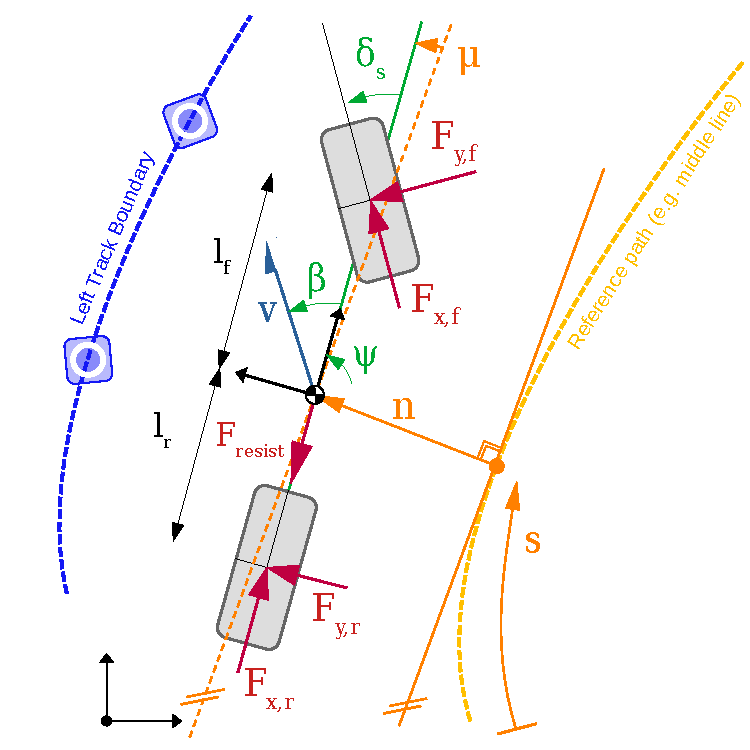
\includegraphics[width=0.7\textwidth]{dyn_bicycle_model.pdf}
	\caption{Dynamic Bicycle Model in curvilinear coordinates}
\end{figure}

\section{Control Approach Decision}

Due to the importance of constraint satisfaction, and because this is one of the outstanding features of Model Predictive Control, we have decided to implement MPC for longitudinal and lateral vehicle control.

\chapter{MPC Formulation: implementation using ACADOS solver}

Although AMZ has maintained a good relationship to Embotech, which is a company that provides real-time nonlinear MPC solvers, we wanted to see if the Open Source project, ACADOS, can provide equally good solvers for our application. To this end, we will now formulate the MPC optimal control problem for the autonomous driving task in the ACADOS framework given in Appendix~\ref{acados_ocp_nlp_formulation}.

\section{Model}

\subsection{Dynamic Model}

The state vector of the MPC model is given by:

\begin{equation}
	\mathbf{x}(t) =
	\left[\begin{array}{c}

		s \\

		n \\

		\mu \\

		{}_Vv_x \\

		{}_Vv_y \\

		\dot{\psi}\;\;\;

	\end{array}\right]
\end{equation}

And the ODE then subsequently as:

\begin{equation}
	f_{expl,\;dyn}(\mathbf{x}, \mathbf{u}) =
	\left[\begin{array}{c}

		\dot{s} \\

		\dot{n} \\

		\dot{\mu} \\

		{}_V\dot{v}_x \\

		{}_V\dot{v}_y \\

		\ddot{\psi}\;\;\;

	\end{array}\right] =
	\left[\begin{array}{c}

		\frac{{}_V v_x \cos(\mu) \,-\, {}_V v_y \sin(\mu)}{1 - n \kappa(s)} \\

		{}_V v_x \sin(\mu) + {}_V v_y \cos(\mu) \\

		\dot{\psi} - \kappa(s)\;\frac{{}_V v_x \cos(\mu) \,-\, {}_V v_y \sin(\mu)}{1 - n \kappa(s)} \\

		\frac{1}{m}  \left( \frac{1}{2} \, F_{x, m} \left[1 + \cos(\delta_s)\right] - F_{y, f} \sin(\delta_s) - F_{resist} \right) + \dot{\psi}\;\cdot {}_V v_y \\

		\frac{1}{m}  \left( F_{y, f} \cos(\delta_s) + F_{y, r} + \frac{1}{2} \, F_{x, m} \sin(\delta_s) \right) - \dot{\psi}\;\cdot {}_V v_x \\

		\frac{1}{I_z}  \left( \frac{1}{2} \, F_{x, m} \sin(\delta_s) l_f + F_{y, f} \cos(\delta_s) l_f - F_{y, r} l_r \right)
	\end{array}\right]
\end{equation}

\begin{equation}
	f_{expl,\;dyn}(\mathbf{x}, \mathbf{u}) =
	\left[\begin{array}{c}

		\dot{s} \\

		\dot{n} \\

		\dot{\mu} \\

		{}_V\dot{v}_y \\

		\ddot{\psi}\;\;\;

	\end{array}\right] =
	\left[\begin{array}{c}

		{}_V v_x\\

		{}_V v_x \cdot \mu + {}_V v_y \\

		\dot{\psi} - \kappa(s)\;\cdot {}_V v_x  \\

		\frac{1}{m}  \left( F_{y, f} + F_{y, r} \right) - \dot{\psi}\;\cdot {}_V v_x \\

		\frac{1}{I_z}  \left(  F_{y, f} \cdot l_f - F_{y, r} \cdot l_r \right)
	\end{array}\right]
\end{equation}

subject to:\\

Resistive Force
\begin{align}
	F_{x, fric} &= C_r \\
	F_{x, drag} &= C_{d} \cdot {}_V v^2_x \\
	F_{resist} &= F_{x, fric} + F_{x, drag}
\end{align}

Slip Angles
\begin{equation}
	\alpha_f = \arctan2\left(\frac{{}_Vv_y + \dot{\psi} l_f}{{}_Vv_x}\right) - \delta_s
	\hspace{2cm}
	\alpha_r = \arctan2\left(\frac{{}_Vv_y - \dot{\psi} l_r}{{}_Vv_x}\right)
\end{equation}

Lateral Pacejka Magic Formula
\begin{align}
	F_{y, f} &= F_{z, f} \; D_{tire} \sin\left(C_{tire} \arctan(B_{tire}\alpha_f)\right) \\
	F_{y, r} &= F_{z, r} \; D_{tire} \sin\left(C_{tire} \arctan(B_{tire}\alpha_r)\right)
\end{align}

Longitudinal and lateral accelerations (in the vehicle frame)
\begin{align}
	{}_V a_x &= {}_V\dot{v}_x - \dot{\psi} \cdot {}_V v_y \\
	{}_V a_y &= {}_V\dot{v}_y + \dot{\psi} \cdot {}_V v_x
\end{align}

Vertical (Normal) Forces
\begin{align}
	F_{z, f} &= m g \frac{l_r}{l_r+l_f}\\
	F_{z, r} &= m g \frac{l_f}{l_r+l_f}
\end{align}

\subsection{Kinematic Model}

For the kinematic model, we only adjust the right hand sides of the explicit dynamic ODE described before for ${}_Vv_x$, ${}_Vv_y$, and $\dot{\psi}$.

\begin{equation}
	f_{expl,\;kin}(\mathbf{x}, \mathbf{u}) =
	\left[\begin{array}{c}

		\dot{s} \\

		\dot{n} \\

		\dot{\mu} \\

		{}_V\dot{v}_x \\

		{}_V\dot{v}_y \\

		\ddot{\psi}\;\;\; \\

		\dot{F}_{x,m} \\

		\dot{\delta}_s

	\end{array}\right] =
	\left[\begin{array}{c}

		\frac{{}_V v_x \cos(\mu) \,-\, {}_V v_y \sin(\mu)}{1 - n \kappa(s)} \\

		{}_V v_x \sin(\mu) + {}_V v_y \cos(\mu) \\

		\dot{\psi} - \kappa(s)\;\frac{{}_V v_x \cos(\mu) \,-\, {}_V v_y \sin(\mu)}{1 - n \kappa(s)} \\

		\frac{1}{m}  \left( F_{x, m} - F_{resist} \right)\\

		\left( \dot{\delta}_{s,u} \cdot {}_Vv_x + \delta_s \cdot \frac{1}{m} F_{x, m}  \right) \cdot  \frac{l_r}{l_r+l_f}\\

		\left( \dot{\delta}_{s,u} \cdot {}_Vv_x + \delta_s \cdot \frac{1}{m} F_{x, m} \right) \cdot  \frac{1}{l_r+l_f} \\

		\dot{F}_{x,m,u} \\

		\dot{\delta}_{s,u}
	\end{array}\right]
\end{equation}


\subsection{Model Combination}

Given a kinematic model and a dynamic model, we blend between them by introducing a blending factor $\gamma_{blend}\in\left[0,\;1\right]$ and computing the convex combination of both right hand sides.

\begin{equation}
	\dot{\mathbf{x}}(t) = f_{expl}(\mathbf{x}, \mathbf{u}) = \gamma_{blend} \cdot f_{expl,\;dyn}(\mathbf{x}, \mathbf{u}) + (1 - \gamma_{blend}) \cdot f_{expl,\;kin}(\mathbf{x}, \mathbf{u})
\end{equation}

Switching between the models is then done based on e.g. lateral acceleration or longitudinal velocity.

\subsection{Algebraic States}

Since \acados{} lets us introduce algebraic variables $\mathbf{z}(t)$, we make use of them to store stage-dependent information that would otherwise not occur in the state. One example is the reference path curvature. Given a (at compile time) fixed vector $\mathbf{s}_{ref} \in \mathbb{R}^{n_{\kappa}}$, we define a differentiable lookup table from the current state $s$ to $\kappa_{LUT}(s)$, where $\mathbf{\kappa}_{ref}\in \mathbb{R}^{n_{\kappa}}$ is the corresponding vector for the curvature values ahead and is defined in the ROS-node as a parameter to the MPC.\\
Finally, the slip angles are also defined as algebraic states for easy access.\\
The algebraic state vector follows as

\begin{equation}
	\mathbf{z}(t) = f_{expl, \mathbf{z}}(\mathbf{x}, \mathbf{u})
	\left[\begin{array}{c}
		\kappa_{LUT} \\
		\alpha_f \\
		\alpha_r
	\end{array}\right]
\end{equation}

\subsection{The full dynamic model}

Finally, we concatenate the differential and algebraic state vectors and make use of the implicit dynamics formulation of \acados{}. Here we also make the dependence on the parameters $\mathbf{p}$ explicit.

\begin{equation}
	0 = f_{impl}(\mathbf{x}(t), \dot{\mathbf{x}}(t), \mathbf{u}(t), \mathbf{z}(t), \mathbf{p}) =
	\left[\begin{array}{c}
		\dot{\mathbf{x}}(t) - f_{expl}(\mathbf{x}, \mathbf{u}, \mathbf{p}) \\
		\mathbf{z}(t) - f_{expl, \mathbf{z}}(\mathbf{x}, \mathbf{u})
	\end{array}\right]
\end{equation}

% ================================================================

\section{Inequality Constraints}

\subsection{Nonlinear Stage Constraints}

We define in total 8 nonlinear inequality constraints, of which 7 are slacked.\\
The first two are tire ellipse constraints for the front and rear wheel respectively:

\begin{align}
	\left( \frac{F_{y, f}} {F_{z, f} D_{tire} \epsilon_{y, f}} \right)^2
	+ \left(\frac{F_{x,m}}{2} \cdot \frac{\epsilon_{x, f}}{F_{z, f} D_{tire} \epsilon_{y, f}} \right) ^2
	- 1
	&\leq s_{u,h,TE,f} \\
	\left( \frac{F_{y, r}} {F_{z, r} D_{tire} \epsilon_{y, r}} \right)^2
	+ \left(\frac{F_{x,m}}{2} \cdot \frac{\epsilon_{x, r}}{F_{z, r} D_{tire} \epsilon_{y, r}} \right) ^2
	- 1
	&\leq s_{u,h,TE,r}
\end{align}

where $D_{tire} \epsilon_{y, f} = \epsilon_{max, f}$ and $D_{tire} \epsilon_{y, r} = \epsilon_{max, r}$.\\
Following the tire constraints, we have four nonlinear inequalities that, in a slacked fashion, make sure the car stays on the track. Based on the heading difference angle $\mu$, we first define three bound variables corresponding to the front, rear, and width dimension of the car.

\begin{align}
	b_f &= L_F \cdot \sin(\mu) \\
	b_r &= L_R \cdot \sin(\mu) \\
	b_w &= \frac{W}{2} \cdot \cos(\mu)
\end{align}

From these definitions, we can formulate the following three inequality constraints, where $n_{\min} < 0$ and $n_{\max}>0$ define the track bounds (possibly based on $s$?).

\begin{align}
	n + b_f + b_w - n_{\max} &\leq s_{u,h,n,fl} \\
	n - b_f + b_w - n_{\max} &\leq s_{u,h,n,rl} \\
	- n - b_f + b_w + n_{\min} &\leq s_{u,h,n,fr} \\
	- n + b_f + b_w + n_{\min} &\leq s_{u,h,n,rr}
\end{align}

The seventh nonlinear inequality constraint is \textbf{not slacked}. It relates the curvature with the lateral deviation from track.

\begin{equation}
	\kappa \cdot n - 1 \leq 0
\end{equation}

To give some sort of bound on velocity along the planning stages, we introduce a (weakly) slacked upper bound on the longitudinal velocity ${}_Vv_x$.

\begin{equation}
	{}_Vv_x - {}_Vv_{x, \max} \leq s_{u,h,vx,rr}
\end{equation}

\subsection{Nonlinear Terminal Constraints}

Except for one upper bound, the terminal constraints are the same as the nonlinear stage constraints. The terminal velocity is reduced for this stage as we want to prevent too optimistic planning which could reduce our recursive feasibility properties.

\subsection{Linear Stage and Terminal Constraints}

For the linear stage and terminal constraints, we only loosely restrict the state variables.


\section{Cost function}
\begin{center}
	\begin{equation}
		J_{MPC}(\textbf{x}_t, \textbf{u}_t) = -\dot{s}_t + (\textbf{x} - \textbf{x}_{ref})^T Q (\textbf{x} - \textbf{x}_{ref}) + \textbf{u}^T R \textbf{u} + S(\textbf{x})
	\end{equation}
\end{center}

% ===========================APPENDIX======================================================

\begin{appendices}

\chapter{\acados{} OCP (Optimal Control Problem) Formulation} \label{acados_ocp_nlp_formulation}

\section{Problem Formulation}\label{sec:problem}
%
\acados{} can handle the following optimization problem
%
\begin{align}
	% cost
	&&&\mathComment{Cost function, see section \ref{sec:cost}}\nonumber\\
	&\underset{\begin{subarray}{c}
			x(\cdot),\,u(\cdot), \, z(\cdot), \, s(\cdot), \, s\terminal
	\end{subarray}}{\min}
	&&\int_0^T l(x(\tau), u(\tau), z(\tau), p)
	+ \frac{1}{2} \matr{s\Lower(\tau) \\ s\upper(\tau) \\ 1} \tran
	\matr{ Z\Lower & 0 & z\Lower \\
		0 & Z\upper & z\upper \\
		{z\Lower}\tran & {z\upper}\tran & 0}
	\matr{s\Lower(\tau) \\ s\upper(\tau) \\ 1} \mathrm{d}\tau \; + \nonumber\\
	&&& \quad \quad m(x(T), z(T), p) +
	\frac{1}{2} \matr{s\Lower\terminal \\ s\upper\terminal \\ 1} \tran
	\matr{ Z\Lower\terminal & 0 & z\Lower\terminal \\
		0 & Z\upper\terminal & z\upper\terminal \\
		{z\Lower\terminal}\tran & {z\upper\terminal}\tran & 0}
	\matr{s\Lower\terminal \\ s\upper\terminal \\ 1}
	\label{eq:cost}\\
	% constraints
	&&&\mathComment{Initial values, see section \ref{sec:constraints:initial}}\nonumber\\
	&\,\,\,\quad \text{s.t.}    &&\underline{x}_0 \leq J_{\textrm{bx},0} \, x(0) \leq \bar{x}_0 , && \label{eq:constraints:initial}\\[1ex]
	&&&\mathComment{Dynamics, see section \ref{sec:dynamics}}\nonumber\\
	%% dynamics
	&&& f\ind{impl}(x(t), \dot{x}(t), u(t), z(t),p ) = 0, &&\quad t \in [0,\,T), \label{eq:dynamics}\\[1ex]
	&&&\mathComment{Path constraints with lower bounds, see section \ref{sec:constraints:path}}\nonumber\\
	%% path constraints with lower slack
	&&&\underline{h} \leq h(x(t), u(t), p) + J_{\textrm{sh}} \, s\lowerh(t), &&\quad t \in [0,\,T),\label{eq:constraints:path:lower_bounds:start}\\
	&&&\underline{x} \leq J_{\textrm{bx}} \, x(t) + J_{\textrm{sbx}} \,s\lowerbx(t), &&\quad t \in (0,\,T),\\
	&&&\underline{u} \leq J_{\textrm{bu}} \,u(t) + J_{\textrm{sbu}} \,s\lowerbu(t), &&\quad t \in [0,\,T),\\
	&&&\underline{g} \leq C\,x(t) + D\,u(t) + J_{\textrm{sg}} \,s\lowerg(t), &&\quad t \in [0,\,T), \\
	&&& s\lowerh (t), s\lowerbx(t), s\lowerbu(t), s\lowerg(t) \geq 0, &&\quad t \in [0,\,T), \label{eq:constraints:path:lower_bounds:end}\\[1ex]
	&&&\mathComment{Path constraints with upper bounds, see section \ref{sec:constraints:path}}\nonumber\\
	%% path constraints with upper slack
	&&& h(x(t), u(t), p) - J_{\textrm{sh}} \, s\upperh(t) \leq \bar{h}, &&\quad t \in [0,\,T),\label{eq:constraints:path:upper_bounds:start}\\
	&&& J_{\textrm{bx}} x(t) - J_{\textrm{sbx}}\, s\upperbx(t) \leq \bar{x}, &&\quad t \in (0,\,T),\\
	&&& J_{\textrm{bu}} u(t) - J_{\textrm{sbu}}\, s\upperbu(t)\leq \bar{u}, &&\quad t \in [0,\,T),\\
	&&&Cx(t) + Du(t) - J_{\textrm{sg}}\, s\upperg \leq \bar{g}, &&\quad t \in [0,\,T), \\
	&&& s\upperh(t), s\upperbx(t), s\upperbu(t), s\upperg(t) \geq 0, &&\quad t \in [0,\,T), \label{eq:constraints:path:upper_bounds:end}\\[1ex]
	%% lower terminal constraints
	&&&\mathComment{Terminal constraints with lower bounds, see section \ref{sec:constraints:terminal}}\nonumber\\
	&&&\underline{h}\terminal \leq h\terminal(x(T), p) + J\ind{sh}\terminal\, s\lowerh\terminal, &&\label{eq:constraints:terminal:lower_bounds:start}\\
	&&&\underline{x}\terminal \leq J_{\textrm{bx}}\terminal\, x(T) + J\ind{sbx}\terminal\, s\lowerbx\terminal, &&\\ % TODO: add Jsbx_e?!
	&&&\underline{g}\terminal \leq C\terminal\, x(T) + J\ind{sg}\terminal\, s\lowerg\terminal \leq \bar{g}\terminal, && \\
	&&& s\lowerh\terminal, s\lowerbx\terminal, s\lowerbu\terminal, s\lowerg\terminal \geq 0, \label{eq:constraints:terminal:lower_bounds:end}\\[1ex]
	%% upper terminal constraints
	&&&\mathComment{Terminal constraints with upper bound, see section \ref{sec:constraints:terminal}}\nonumber\\
	&&& h\terminal(x(T), p) - J\ind{sh}\terminal\, s\ind{u,h}\terminal \leq \bar{h}\terminal, &&\label{eq:constraints:terminal:upper_bounds:start}\\
	&&& J_{\textrm{bx}}\terminal\, x(T) - J\ind{sbx}\terminal\, s\ind{u,bx}\terminal \leq \bar{x}^{e}, &&\\ % TODO: add Jsbx_e?!
	&&& C\terminal\, x(T) - J\ind{sg}\terminal\, s\ind{u,g}\terminal \leq \bar{g}\terminal \\
	&&& s\upperh\terminal, s\upperbx\terminal, s\upperbu\terminal, s\upperg\terminal \geq 0,\label{eq:constraints:terminal:upper_bounds:end}
\end{align}
%
with
\begin{itemize}
	\item state vector $ x: \R \rightarrow \R^{\nx} $
	\item control vector $ u: \R \rightarrow \R^{\nuu} $
	\item algebraic state vector $ z: \R \rightarrow \R^{\nz} $
	\item model parameters $ p \in \R^{\np} $
	\item slacks for path constraints $ s\Lower(t) = (s\lowerbu, s\lowerbx, s\lowerg, s\lowerh) \in \R^{\ns} $ and $ s\upper(t) = (s\upperbu, s\upperbx, s\upperg, s\upperh) \in \R^{\ns} $
	\item slacks for terminal constraints $ s\Lower\terminal(t) = (s\lowerbx\terminal, s\lowerg\terminal, s\lowerh\terminal) \in \R^{\ns\terminal} $ and $ s\upper\terminal(t) = (s\upperbx\terminal, s\upperg\terminal, s\upperh\terminal) \in \R^{\ns\terminal} $
\end{itemize}
%
Some of the following restrictions may apply to matrices in the formulation:
\begin{center}
	\begin{tabular}{ll}
		\textbf{DIAG} & diagonal\\
		\textbf{SPUM} & horizontal slice of a permuted unit matrix\\
		\textbf{SPUME} & like \textbf{SPUM}, but with empty rows intertwined
	\end{tabular}
\end{center}
%
\paragraph{Document Purpose}
This document is only associated to the \matlab{} interface of \acados.
Here, the focus is to give a mathematical overview of the problem formulation and possible options to model it within \acados.
The problem formulation and the possibilities of \acados{} are similar in the \python{} interface, however, some of the string identifiers are different.
The documentation is not exhaustive and does not contain a full description for the \matlab{} interface.

You can find examples int the directory \code{<acados>/examples/acados\_matlab\_octave}.
The source code of the \acados{} \matlab{} interface is found in: \code{<acados>/interfaces/acados\_matlab\_octave} and should serve as a more extensive, complete and up-to-date documentation about the possibilities.
%
\section{Dynamics}\label{sec:dynamics}
%
The system dynamics term is used to connect state trajectories from adjacent shooting nodes by means of equality constraints.
%
The system dynamics equation~\eqref{eq:dynamics} is replaced with a discrete-time dynamic system.
The dynamics can be formulated in different ways in \acados:
As implicit equations in continuous time~\eqref{eq:dynamics:implicit}, or as explicit equations in continuous time~\eqref{eq:dynamics:explicit} or directly as discrete-time dynamics \eqref{eq:dynamics:discrete}.
This section and table~\ref{tab:dynamics} summarizes the options.
%
\subsection{Implicit Dynamics}\label{sec:dynamics:implicit}
%
The most general way to provide a continuous time ODE in \acados\ is to define the function $ f\ind{impl}: \mathbb{R}^{\nx}\times\mathbb{R}^{\nx}\times\mathbb{R}^{\nuu}\times\mathbb{R}^{\nz}\times\mathbb{R}^{\np} \rightarrow \mathbb{R}^{\nx+\nz}$ which is fully implicit DAE formulation describing the system as:
\begin{align}
	f\ind{impl}(x, \dot{x}, u, z, p) &= 0.\label{eq:dynamics:implicit}
\end{align}
\acados{} can discretize $ f\ind{impl} $ with a classical implicit Runge-Kutta (\code{irk}) or a structure exploiting implicit Runge-Kutta method (\code{irk\_gnsf}). Both discretization methods are set using the \code{'sim\_method'} identifier in a \code{acados\_ocp\_opts} class instance.

%
\subsection{Explicit Dynamics}\label{sec:dynamics:explicit}
%
Alternatively, \acados{} offers an explicit Runge-Kutta integrator (\code{erk}), which can be used with explicit ODE models, i.e., models of the form
\begin{align}
	f\ind{expl}(x,u,p) &= \dot{x}.\label{eq:dynamics:explicit}
\end{align}
%
\subsection{Discrete Dynamics}\label{sec:dynamics:discrete}
%
Another option is to provide a discrete function that maps state $x_i$, control $u_i$ and parameters $p_i$ from shooting node~$i$ to the state $x_{i+1}$ of the next shooting node $i+1$, i.e., a function
\begin{align}
	x_{i+1} &= f\ind{disc}(x_i,u_i,p_i).\label{eq:dynamics:discrete}
\end{align}
%
\begin{table}[h!]
	\centering
	\caption{Dynamics definitions} \label{tab:dynamics}
	\begin{tabular}{cccc}
		\toprule
		Term & String identifier & Data type & Required \\ \midrule
		$ f\ind{impl} $ respectively $ f\ind{expl} $ & \code{dyn\_expr\_f}    & \casadi~expression & \mandatory \\
		$f\ind{disc}$ & \code{dyn\_exp\_phi} & \casadi~expression & \mandatory \\
		- & \code{dyn\_type}    & string (\str{explicit}, \str{implicit} or \str{discrete}) & \mandatory \\
		\bottomrule
	\end{tabular}
\end{table}
%
\section{Cost}\label{sec:cost}
%
There are different \acados~modules to model the cost functions in equation~\eqref{eq:cost}.
\begin{itemize}
	\item $ l: \mathbb{R}^{\nx}\times\mathbb{R}^{\nuu}\times\mathbb{R}^{\nz} \rightarrow \mathbb{R}$ is the Lagrange objective term.
	\item $ m: \mathbb{R}^{\nx}\times\mathbb{R}^{\nz} \rightarrow \mathbb{R} $ is the Mayer objective term.
\end{itemize}
to define which one is used set \code{cost\_type} for $l$, \code{cost\_type\_e} for $m$.

Setting the slack penalties in equation~\eqref{eq:cost} is done in the same way for all cost modules, see table~\ref{tab:cost:slack} for an overview.
%
\begin{table}[h!]
	\centering
	\caption{Cost module slack variable options} \label{tab:cost:slack}
	\begin{tabular}{cccc}
		\toprule
		Term  & String id & Data type & Required \\ \midrule
		$ Z\Lower $          & \code{cost\_Zl}    & double, \textbf{DIAG}  & \optional \\
		$ Z\upper $          & \code{cost\_Zu}    & double, \textbf{DIAG}  & \optional   \\
		$ z\Lower $          & \code{cost\_zl}    & double  & \optional   \\
		$ z\upper $          & \code{cost\_zu}    & double  & \optional   \\ [1em]
		$ Z\Lower\terminal $ & \code{cost\_Zl\_e} & double, \textbf{DIAG} & \optional   \\
		$ Z\upper\terminal $ & \code{cost\_Zu\_e} & double, \textbf{DIAG} & \optional   \\
		$ z\Lower\terminal $ & \code{cost\_zl\_e} & double  & \optional   \\
		$ z\upper\terminal $ & \code{cost\_zu\_e} & double  & \optional   \\
		\bottomrule
	\end{tabular}
\end{table}
%
Moreover, you can specify \code{cost\_Z}, to set $ Z\Lower$, $Z\upper$ to the same values, i.e., use a symmetric L2 slack penalty.
Similarly, \code{cost\_z}, \code{cost\_Z\_e}, \code{cost\_z\_e} can be used to set symmetric slack L1 penalties, respectively penalties for the terminal slack variables.

Note, that the dimensions of the slack variables $s\Lower(t)$, $s\Lower\terminal(t)$, $s\upper(t)$ and $s\upper\terminal(t)$ are determined by \acados{} from the associated matrices ($Z\Lower$, $Z\upper$,  $J\ind{sh}$, $J\ind{sg}$, $J\ind{sbu}$, $J\ind{sbx}$ etc.).
%
\subsection{Cost module: \code{auto}}\label{sec:cost:auto}
%
Set \code{cost\_type} to \code{auto} (default).
In this case \acados{} detects if the cost function specified is a linear least squares term and transcribes it in the corresponding form.
Otherwise, it is formulated using the external cost module.
Note: slack penalties are optional and we plan to detected them from the expressions in future versions.
Table~\ref{tab:cost:auto} shows the available options.
%
\begin{table}[h!]
	\centering
	\caption{Cost module \code{auto} options} \label{tab:cost:auto}
	\begin{tabular}{cccc}
		\toprule
		Term & String identifier & Data type & Required \\ \midrule
		$ l $ & \code{cost\_expr\_ext\_cost}    & \casadi~expression   & \mandatory  \\
		%        $ m $ & \code{cost\_expr\_ext\_cost\_e}    & \casadi~expression  & \mandatory \\
		\bottomrule
	\end{tabular}
\end{table}
%
\subsection{Cost module: \code{external}}\label{sec:cost:external}
%
Set \code{cost\_type} to \code{ext\_cost}.
See table~\ref{tab:cost:external} for the available options.
\begin{table}[h!]
	\centering
	\caption{Cost module \code{external} options} \label{tab:cost:external}
	\begin{tabular}{cccc}
		\toprule
		Term & String identifier & Data type & Required \\ \midrule
		$ l $ & \code{cost\_expr\_ext\_cost}    & \casadi~expression   & \mandatory  \\
		$ m $ & \code{cost\_expr\_ext\_cost\_e}    & \casadi~expression  & \mandatory \\
		\bottomrule
	\end{tabular}
\end{table}
%
\subsection{Cost module: \code{linear least squares}}\label{sec:cost:linear_ls}
%
In order to activate the \code{linear least squares} cost module, set \code{cost\_type} to \code{linear\_ls}.\\
The Lagrange cost term has the form
\begin{align}
	l(x, u, z) &= \frac{1}{2} \norm{ \underbrace{V_x\, x + V_u\, u + V_z\, z}_{\displaystyle y} - y\ind{ref}}_W^2 \label{eq:cost:linear_ls:l}
\end{align}
where matrices $ V_x \in \mathbb{R}^{n_y \times n_x}$, $V_u \in \mathbb{R}^{n_y \times n_u}$ are $V_z \in \mathbb{R}^{n_y \times n_z}$ map $x$, $u$ and $z$ onto $y$, respectively and $W \in \mathbb{R}^{n_y \times n_y}$ is the weighing matrix. The vector $y\ind{ref} \in \mathbb{R}^{n_y}$ is the reference.

Similarly, the Mayer cost term has the form
\begin{align}
	m(x, u, z) &= \frac{1}{2} \norm{ \underbrace{V_x\terminal x}_{\displaystyle y\terminal} - y\ind{ref}\terminal}_{W\terminal}^2 \label{eq:cost:linear_ls:m}
\end{align}
where matrix $ V\terminal_x \in \mathbb{R}^{n_{y\terminal} \times n_x}$ maps $x$ onto $y\terminal$ and $W\terminal \in \mathbb{R}^{n_{y\terminal} \times n_{y\terminal}}$ is the weighing matrix. The vector $y\terminal_\textrm{ref} \in \mathbb{R}^{n_{y\terminal}}$ is the reference.

See table~\ref{tab:cost:linear_ls} for the available options of this cost module.
%
\begin{table}[h!]
	\centering
	\caption{Cost module \code{linear\_ls} options} \label{tab:cost:linear_ls}
	\begin{tabular}{cccc}
		\toprule
		Term & String identifier & Data type & Required \\ \midrule
		$ V_x $ & \code{cost\_Vx}    & double & \mandatory   \\
		$ V_u $ & \code{cost\_Vu}    & double & \mandatory   \\
		$ V_z $ & \code{cost\_Vz}    & double & \mandatory  \\
		$ W $ & \code{cost\_W}    & double & \mandatory  \\
		$ y\ind{ref} $ & \code{cost\_y\_ref}    & double & \mandatory   \\ [1em]
		$ V_x\terminal $ & \code{cost\_Vx\_e}    & double  & \mandatory  \\
		$ W\terminal $ & \code{cost\_W\_e}    & double & \mandatory   \\
		$ y\ind{ref}\terminal $ & \code{cost\_y\_ref\_e}   & double & \mandatory   \\
		\bottomrule
	\end{tabular}
\end{table}
%
\subsection{Cost module: \code{nonlinear least squares}}\label{sec:cost:nonlinear_ls}
%
In order to activate the \code{nonlinear least squares} cost module, set \code{cost\_type} to \code{nonlinear\_ls}.

The \code{nonlinear least squares} cost function has the same basic form as eqns.~(\ref{eq:cost:linear_ls:l}~-~\ref{eq:cost:linear_ls:m}) of the \code{linear least squares} cost module.
The only difference is that $ y $ and $ y\terminal $ are defined by means of \casadi{} expressions, instead of via matrices $ V_x $, $ V_u $, $ V_z $ and $ V_x\terminal $.
%
See table~\ref{tab:cost:nonlinear_ls} for the available options of this cost module.
%
\begin{table}[h!]
	\centering
	\caption{Cost module \code{nonlinear\_ls} options} \label{tab:cost:nonlinear_ls}
	\begin{tabular}{cccc}
		\toprule
		Term & String identifier & Data type & Required \\ \midrule
		$ y $ & \code{cost\_expr\_y}    & \casadi~expression  & \mandatory   \\
		$ W $ & \code{cost\_W}    & double  & \mandatory   \\
		$ y\ind{ref} $ & \code{cost\_y\_ref}    & double & \mandatory    \\ [1em]
		$ y\terminal $ & \code{cost\_expr\_y\_e}    & \casadi~expression  & \mandatory   \\
		$ W\terminal $ & \code{cost\_W\_e}    & double & \mandatory   \\
		$ y\ind{ref}\terminal $ & \code{cost\_y\_ref\_e}    & double  & \mandatory   \\
		\bottomrule
	\end{tabular}
\end{table}
%
%\newpage
\section{Constraints}\label{sec:constraints}
%
This section is about how to define the constraints equations \eqref{eq:constraints:initial} and (\ref{eq:constraints:path:lower_bounds:start} - \ref{eq:constraints:terminal:upper_bounds:end}).

The \matlab{} interface supports the constraint module \code{bgh}, which is able to handle simple \textbf{b}ounds (on $ x $ and $ u $), \textbf{g}eneral linear constraints and general nonlinear constraints.
Meanwhile, the \python{} interface also supports the \acados{} constraint module \code{bgp}, which can handle convex-over-nonlinear constraints in a dedicated fashion.
%
\subsection{Initial State}\label{sec:constraints:initial}
%
Note: An initial state is not required.
For example for moving horizon estimation (MHE) problems it should not be set.

Two possibilities exist to define the initial states equation~\eqref{eq:constraints:initial}: a simple syntax and an extended syntax.

\paragraph{Simple syntax}
defines the full initial state $x(0)=\bar{x}_0$. The options are found in table~\ref{tab:constraints:simplesyntax}.
\begin{table}[h!]
	\centering
	\caption{Simple syntax for setting the initial state} \label{tab:constraints:simplesyntax}
	\begin{tabular}{cccc}
		\toprule
		Term & String identifier & Data type & Required \\ \midrule
		$ \bar{x}_0 $ & \code{constr\_x0} & double & \optional \\
		\bottomrule
	\end{tabular}
\end{table}
%
\paragraph{Extended syntax}
allows to define upper and lower bounds on a subset of states.
The options for the extended syntax are found in table~\ref{tab:constraints:extendedsyntax}.
\begin{table}[h!]
	\centering
	\caption{Extended syntax for setting the initial state} \label{tab:constraints:extendedsyntax}
	\begin{tabular}{cccc}
		\toprule
		Term & String identifier & Data type & Required \\ \midrule
		$ \underline{x}_0 $ & \code{constr\_lbx\_0} & double & \optional \\
		$ \bar{x}_0 $ & \code{constr\_ubx\_0} & double & \optional \\
		$ J_{\textrm{bx},0} $ & \code{constr\_Jbx\_0} & double & \optional \\
		\bottomrule
	\end{tabular}
\end{table}
%
\subsection{Path Constraints}\label{sec:constraints:path}
%
Table~\ref{tab:constraints:path} shows the options for defining the path constraints equations~(\ref{eq:constraints:path:lower_bounds:start} ~-~\ref{eq:constraints:path:upper_bounds:end}).
Here, matrices
\begin{itemize}
	\item $J\ind{sh}$, maps lower slack vectors $s\ind{l,h}(t)$ and upper slack vectors $s\ind{u,h}(t)$ onto the non-linear constraint expressions $h(x,u,p)$.
	\item $J\ind{bx}$, $J\ind{bu}$ map $x(t)$ and $u(t)$ onto its bounds vectors $\underline{x}$, $\bar{x}$ and $\underline{u}$, $\bar{u}$, respectively.
	\item $J\ind{sx}$, $J\ind{su}$ map lower slack vectors $s\ind{l,bx}(t)$, $s\ind{l,bu}(t)$ and upper slack vectors $s\ind{u,bx}(t)$, $s\ind{u,bu}(t)$ onto $x(t)$ and $u(t)$, respectively.
	\item $J\ind{sg}$ map lower slack vectors $s\ind{l,g}(t)$ and upper slack vectors $s\ind{u,g}(t)$ onto lower and upper equality bounds $\underline{g}$, $\bar{g}$, respectively.
	\item $C$, $D$ map $x(t)$ and $u(t)$ onto lower and upper inequality bounds $\underline{g}$, $\bar{g}$ (polytopic constraints)
\end{itemize}
%
\begin{table}[h!]
	\centering
	\caption{Path constraints options} \label{tab:constraints:path}
	\begin{tabular}{cccc}
		\toprule
		Term & String identifier & Data type & Required \\ \midrule
		$J\ind{bx}$ & \code{constr\_Jbx}    & double, \textbf{SPUM} & \optional  \\
		$\underline{x} $    & \code{constr\_lbx}     & double  & \optional  \\
		$\bar{x} $  & \code{constr\_ubx}     & double  & \optional   \\ [1em]
		$J\ind{bu}$ & \code{constr\_Jbu}    & double, \textbf{SPUM}   & \optional    \\
		$\underline{u} $    & \code{constr\_lbu}     & double   & \optional   \\
		$\bar{u} $         & \code{constr\_ubu}     & double  & \optional   \\ [1em]
		$C$ & \code{constr\_C}    & double  & \optional \\
		$D $    & \code{constr\_D}     & double  & \optional \\
		$\underline{g} $    & \code{constr\_lg}     & double  & \optional    \\
		$\bar{g} $         & \code{constr\_ug}     & double  & \optional   \\ [1em]
		$ h $ & \code{constr\_expr\_h}    & \casadi~expression  & \optional   \\
		$\underline{h} $    & \code{constr\_lh}     & double   & \optional   \\
		$\bar{h} $         & \code{constr\_uh}     & double  & \optional   \\ [1em]
		$ J\ind{sbx} $ & \code{constr\_Jsbx} & double, \textbf{SPUME} & \optional  \\
		$ J\ind{sbu} $ & \code{constr\_Jsbu} & double, \textbf{SPUME}  & \optional \\
		$ J\ind{sg} $ & \code{constr\_Jsg} & double, \textbf{SPUME} & \optional  \\
		$ J\ind{sbx} $ & \code{constr\_Jsh} & double, \textbf{SPUME}  & \optional  \\
		\bottomrule
	\end{tabular}
\end{table}
%
%%%%%%%%%%%%%%%%%%%%%%%%%%%%%%%%%%%%%%%%%
%\newpage
\subsection{Terminal Constraints}\label{sec:constraints:terminal}
%
Table~\ref{tab:constraints:terminal} shows the options for defining the terminal constraints equations~(\ref{eq:constraints:terminal:lower_bounds:start} ~-~\ref{eq:constraints:terminal:upper_bounds:end}).
Here, matrices
\begin{itemize}
	\item $J\ind{sh}\terminal$, maps lower slack vectors $s\ind{l,h}\terminal(t)$ and upper slack vectors $s\ind{u,h}\terminal(t)$ onto non-linear terminal constraint expressions $h\terminal(x(T), p)$.
	\item $J\ind{bx}\terminal$ maps $x(T)$ onto its bounds vectors $\underline{x}\terminal$ and $\bar{x}\terminal$.
	\item $J\ind{sbx}\terminal$ maps lower slack vectors $s\ind{l,bx}\terminal$ and upper slack vectors $s\ind{u,bx}\terminal$ onto $x(T)$.
	\item $J\ind{sg}\terminal$ map lower slack vectors $s\ind{l,g}\terminal(t)$ and upper slack vectors $s\ind{u,g}\terminal(t)$ onto lower and upper equality bounds $\underline{g}\terminal$, $\bar{g}\terminal$, respectively.
	\item $C\terminal$ maps $x(T)$ onto lower and upper inequality bounds $\underline{g}\terminal$, $\bar{g}\terminal$ (polytopic constraints)
\end{itemize}
%
\begin{table}[h!]
	\centering
	\caption{Terminal constraints options} \label{tab:constraints:terminal}
	\begin{tabular}{cccc}
		\toprule
		Term & String identifier & Data type & Required \\ \midrule
		$J\ind{bx}\terminal$ & \code{constr\_Jbx\_e}    & double, \textbf{SPUM}   & \optional   \\
		$\underline{x}\terminal $    & \code{constr\_lbx\_e}     & double  & \optional   \\
		$\bar{x}\terminal $         & \code{constr\_ubx\_e}     & double   & \optional  \\ [1em]
		$ C\terminal $ & \code{constr\_C\_e}    & double   & \optional   \\
		$\underline{g}\terminal $    & \code{constr\_lg}     & double   & \optional   \\
		$\bar{g}\terminal $         & \code{constr\_ug}     & double   & \optional  \\ [1em]
		$ h\terminal $ & \code{constr\_expr\_h\_e}    & \casadi~expression   & \optional  \\
		$\underline{h}\terminal $    & \code{constr\_lh\_e}     & double   & \optional   \\
		$\bar{h}\terminal $         & \code{constr\_uh\_e}     & double  & \optional   \\ [1em]
		$ J\ind{sbx}\terminal $ & \code{constr\_Jsbx} & double, \textbf{SPUME}   & \optional \\
		$ J\ind{sg}\terminal $ & \code{constr\_Jsg\_e} & double, \textbf{SPUME} & \optional  \\
		$ J\ind{sbx}\terminal $ & \code{constr\_Jsh\_e} & double, \textbf{SPUME}  & \optional  \\
		\bottomrule
	\end{tabular}
\end{table}
%
\section{External links}\label{sec:external_links}
%
A table sheet with additional info is found here:\newline
\url{https://docs.google.com/spreadsheets/d/1rVRycLnCyaWJLwnV47u30Vokp7vRu68og3OhlDbSjDU/edit?usp=sharing}
%
\section{Model}\label{sec:model}
%
A model instance is created using \code{ocp\_model = acados\_ocp\_model()}. It contains all model definitions for simulation and for usage in the OCP solver.
See table~\ref{tab:model:options} for the available options.
Furthermore, see \code{ocp\_model.model\_struct} to see what other fields can be set via direct access.
%
\begin{table}
	\centering
	\caption{Model \code{set(id, data)} options}
	\label{tab:model:options}
	\begin{tabular}{cccc}
		\toprule
		String id & Data type & Description & Required\\
		\midrule
		\code{name} & string & model name, used for code generation, default: \str{ocp\_model} & \optional \\
		\code{T} & double & end time & \mandatory \\
		\code{sym\_x} & \casadi{} expr. & state vector $x$ in problem formulation in sec.~\ref{sec:problem} & \mandatory \\
		\code{sym\_u} & \casadi{} expr. & control vector $u$ in problem formulation in sec.~\ref{sec:problem} & only in OCP \\
		\code{sym\_xdot} & \casadi{} expr. & derivative of the state $\dot{x}$ in implicit dynamics eq.~\eqref{eq:dynamics} & if IRK is used \\
		\code{sym\_z} & \casadi{} expr. & algebraic state $z$ in implicit dynamics eq.~\eqref{eq:dynamics} & \optional, only with IRK \\
		\code{sym\_p} & \casadi{} expr. & parameters $p$ of the problem formulation in sec.~\ref{sec:problem} & \optional \\
		\multicolumn{4}{c}{$\vdots$}\\
		\multicolumn{4}{c}{Additionally, options from tables \ref{tab:dynamics}, \ref{tab:cost:slack}, \ref{tab:cost:auto}, \ref{tab:cost:external}, \ref{tab:cost:linear_ls}, \ref{tab:cost:nonlinear_ls}, %\ref{tab:constr_type},
			\ref{tab:constraints:simplesyntax}, \ref{tab:constraints:extendedsyntax}, \ref{tab:constraints:path} and \ref{tab:constraints:terminal}, apply here.}\\
		\multicolumn{4}{c}{$\vdots$}\\
		\bottomrule
	\end{tabular}%
\end{table}%
%
\section{Solver \& Options}\label{sec:solver}
%
An instance of the solver options class is created by using: \code{ocp\_opts = acados\_ocp\_opts()}.
Together with the model these options are used when instancing the solver interface class: \code{ocp = acados\_ocp(ocp\_model, ocp\_opts)}.\\
Tables \ref{tab:solver_options}, \ref{tab:solver_options:qp_solver_option} and \ref{tab:solver_options:regularize_method} show (almost) all available options.
These options are set in \matlab{} via \code{ocp\_opts.set(<stringid>, <value>)}.
% Some options are not (yet) implemented in the \code{.set(*)}-interface and can be accessed via a struct by using \code{ocp\_opts.opts\_struct.(<stringid>) = <value>}.
Furthermore, the struct \code{ocp\_opts.opts\_struct} can be used as a reference for what other fields are available.
\\
Note that some options of the solver can be modified after creation using the routine: \code{set(<stringid>, <value>)}.
Some options can only be set before the solver is created, especially options that influence the memory requirements of OCP solver, such as the modules used in the formulation, the QP solver, etc.

%
%\begin{landscape}
\begin{table}
	\centering
	\small
	\caption{Solver options}\label{tab:solver_options}
	\begin{tabulary}{\textwidth}{p{4cm}@{}C@{}C@{}p{10cm}}
		\toprule
		{String identifier} & Type & Default & {Description} \\ \midrule
		\multicolumn{4}{l}{\emph{Code generation}} \\
		\code{compile\_interface} & string & \str{auto} & in (\str{auto}, \str{true}, \str{false}) \\
		\code{codgen\_model} & string & \str{true} & in (\str{true}, \str{false}) \\
		\code{compile\_model} & string & \str{true} & in (\str{true}, \str{false}) \\
		\code{output\_dir} & string & \str{build} & codegen output directory\\
		\midrule

		\multicolumn{4}{l}{\emph{Shooting nodes}} \\
		\code{param\_scheme\_N} & int $>1$ & $10$ & uniform grid: number of shooting nodes; acts together with end time \code{T} from model. \\
		% set one of the following for nonuniform grid
		{\code{shooting\_nodes} or \code{param\_\-scheme\_shooting\_nodes}} & doubles & \code{[]} & nonuniform grid option 1: direct definition of the shooting node times \\
		\code{time\_steps} & doubles & \code{[]} & {nonuniform grid option 2: definition of deltas between shooting nodes}\\
		\midrule

		\multicolumn{4}{l}{\emph{Integrator}} \\
		\code{sim\_method} & string & \str{irk} & \str{erk}, \str{irk}, \str{irk\_gnsf} \\
		\code{sim\_method\_num\_stages} & int & $4$ & Runge-Kutta int.\ stages: ($1$)~RK1, ($2$)~RK2, ($4$)~RK4\\
		\code{sim\_method\_num\_steps} & int & $1$\\
		\code{sim\_method\_newton\_iter} & int & $3$\\
		\code{gnsf\_detect\_struct} & string & \str{true}\\
		\midrule

		\multicolumn{4}{l}{\emph{NLP solver}} \\
		\code{nlp\_solver} & string & \str{sqp} & in (\str{sqp}, \str{sqp\_rti})\\
		\code{nlp\_solver\_max\_iter} & int $>1$ & $100$ & maximum number of NLP iterations\\
		\code{nlp\_solver\_tol\_stat} & double & $10^{-6}$ & stopping criterion \\
		\code{nlp\_solver\_tol\_eq}   & double & $10^{-6}$ & stopping criterion \\
		\code{nlp\_solver\_tol\_ineq} & double & $10^{-6}$ & stopping criterion \\
		\code{nlp\_solver\_tol\_comp} & double & $10^{-6}$ & stopping criterion \\
		\code{nlp\_solver\_ext\_qp\_res} & int & $0$ & compute QP residuals at each NLP iteration \\
		\code{nlp\_solver\_step\_length} & double & $1.0$ & fixed step length in SQP algorithm \\
		\code{rti\_phase} & int & $0$ & RTI phase: ($1$) preparation, ($2$) feedback, ($0$) both \\
		\midrule

		\multicolumn{4}{l}{\emph{QP solver}} \\
		\code{qp\_solver} & string & $\longrightarrow$ & Defines the quadratic programming solver and condensing strategy. See table~\ref{tab:solver_options:qp_solver_option}\\

		\code{qp\_solver\_iter\_max} & int & $50$ & maximum number of iterations per QP solver call\\
		% \code{qp\_solver\_cond\_N} & 5\\ % New horizon after partial condensing
		\code{qp\_solver\_cond\_ric\_alg} & int & $0$ & factorize hessian in the condensing: ($0$) no, ($1$) yes \\
		\code{qp\_solver\_ric\_alg} & int & $0$ & HPIPM specific \\
		\code{qp\_solver\_warm\_start} & int & $0$ & ($0$)~cold start, ($1$)~warm start primal variables, ($2$)~warm start and dual variables \\
		\code{warm\_start\_first\_qp} & int & $0$ & warm start even in first SQP iteration: ($0$)~no, ($1$)~yes \\
		\midrule
		% globalization
		\multicolumn{4}{l}{\emph{globalization}} \\
		\code{globalization} & string & \scriptsize\str{fixed\_step} & globalization strategy in (\str{fixed\_step}, \str{merit\_backtracking}), note \code{merit\_backtracking} is a preliminary implementation.\\
		\code{alpha\_min} & double & $0.05$ & minimum step-size, relevant for globalization  \\
		\code{alpha\_reduction} & double & $0.7$ &  step-size reduction factor, relevant for globalization  \\
		\midrule
		\multicolumn{4}{l}{\emph{Hessian approximation}} \\
		{\code{nlp\_solver\_\-exact\_hessian}} & string & \str{false} & use exact hessian calculation: (\str{})in (\str{true}, \str{false}), use exact \\
		\code{regularize\_method} & string & $\longrightarrow$ & Defines the hessian regularization method. See table~\ref{tab:solver_options:regularize_method}\\
		\code{levenberg\_marquardt} & double & $0.0$ & in case of a singular hessian, setting this $>0$ can help convergence \\
		\code{exact\_hess\_dyn} & int & $1$ & in ($0$, $1$), compute and use hessian in dynamics, only if \str{nlp\_\-solver\_\-exact\_\-hessian} = \str{true} \\
		\code{exact\_hess\_cost} & int & $1$ & in ($0$, $1$), only if \str{nlp\_solver\_exact\_hessian} = \str{true} \\
		\code{exact\_hess\_constr} & int & $1$ & in ($0$, $1$), only if \str{nlp\_solver\_exact\_hessian} = \str{true} \\
		\midrule
		\multicolumn{4}{l}{\emph{Other}} \\
		\code{print\_level} & int $\geq 0$ & $0$ & verbosity of the solver: ($0$) silent, ($>0$) print first QP problems and solution during SQP\\
		\bottomrule
	\end{tabulary}
\end{table}
%
\begin{table}
	\centering
	\caption{Solver \code{set(\str{qp\_solver}, <stringid>)} options. The availability depends on for which solver interfaces \acados{} was linked to.}\label{tab:solver_options:qp_solver_option}
	\begin{tabular}{c@{ }c@{}c}
		\toprule
		Solver lib & Condensing & {String identifier} \\ \midrule
		\multirow{2}{1.2cm}{\centering HPIPM} & partial & \code{partial\_condensing\_hpipm}*\\
		& full & \code{full\_condensing\_hpipm} \\[1ex]
		HPMPC & partial & \code{partial\_condensing\_hpmpc} \\[1ex]
		\multirow{2}{2cm}{\centering OOQP} & partial & \code{partial\_condensing\_ooqp} \\
		& full & \code{full\_condensing\_ooqp} \\[1ex]
		OSQP & partial & \code{partial\_condensing\_osqp} \\
		QORE & full & \code{full\_condensing\_qore} \\
		qpDUNES & partial & \code{partial\_condensing\_qpdunes} \\
		qpOASES & full & \code{full\_condensing\_qpoases} \\
		\bottomrule
		\multicolumn{3}{r}{\footnotesize * default}
	\end{tabular}
\end{table}
%
\begin{table}
	\centering
	\caption{Solver \code{set(\str{regularize\_method}, <stringid>)} options}
	\label{tab:solver_options:regularize_method}
	\begin{tabular}{cc}
		\toprule
		String identifier & Description \\\midrule
		\code{no\_regularize}* & don‘t regularize \\
		\code{mirror} & \href{https://cdn.syscop.de/publications/Verschueren2017.pdf}{see Verschueren2017} \\
		\code{project} & \href{https://cdn.syscop.de/publications/Verschueren2017.pdf}{see Verschueren2017} \\
		\code{project\_reduc\_hess} & preliminary \\
		\code{convexify} & \href{https://cdn.syscop.de/publications/Verschueren2017.pdf}{see Verschueren2017} \\
		\bottomrule
		\multicolumn{2}{r}{\footnotesize * default}
	\end{tabular}
\end{table}

\end{appendices}


\end{document}
